\chapter{Chiamate di Sistema}
\begin{defn}[Chiamata di Sistema]
Interfaccia ai servizi principali, messa a disposizione da il sistema operativo.
Solitamente, queste chiamate sono funzioni scritte in C/C++ o per alcuni casi specifici in linguaggio Assembly.
\end{defn}

\section{Application Programming Interface (API)}
Nei sistemi moderni, vengono eseguite migliaia di system calls ogni secondo, quindi, gli sviluppatori, 
per realizzare le applicazioni si affidano a una \textbf{Application Programming Interface} (\textbf{API}).

\begin{defn}[API]
Insieme di funzioni disponibili per un programmatore di applicazioni,
inclusi i parametri passati a ciascuna funzione e i valori di ritorno che il programmatore può aspettarsi.
\end{defn}

Le API più comuni sono quella di Windows, POSIX (Unix, Linux e MacOS) e quella per la Java Virtual Machine.

\begin{figure}[!htb]
    \centering
    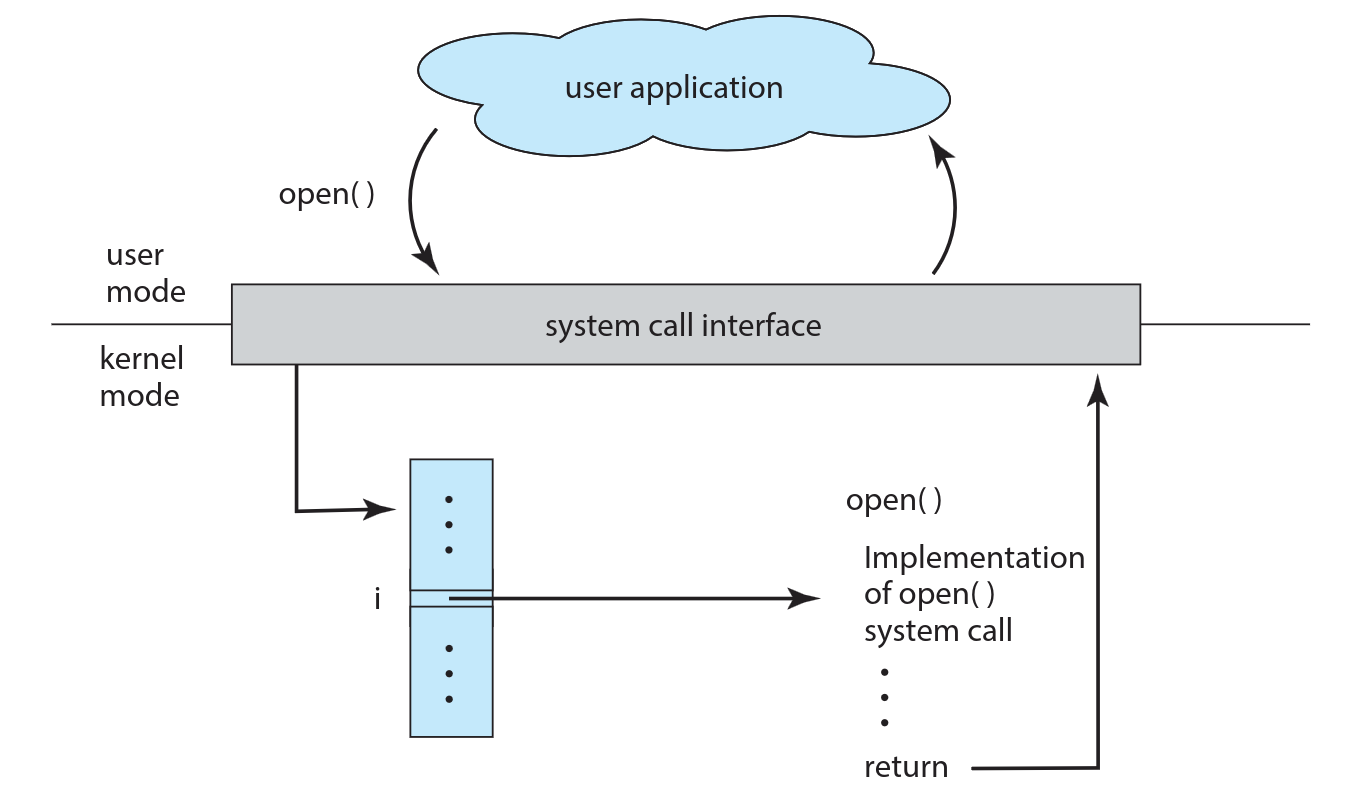
\includegraphics[width=0.8\linewidth]{Images/calls/call.png}
    \caption{Esempio di System Call.}
\end{figure}

Un fattore nella gestione delle chiamate di sistema è l'\textbf{ambiente di esecuzione} (\textbf{RTE}), ossia l'insieme di software necessari per eseguire applicazioni scritte 
in un determinato linguaggio di programmazione, inclusi i relativi compilatori o interpreti, oltre ad altri componenti come librerie e loader.\\
L'RTE, tramite una \textbf{system call interface}, fa da link fra le system call al sistema operativo e le istruzione dell'API. \\
Tipicamente, a ogni chiamata di sistema viene associato un numero e viene mantenuta una tabella indicizzati secondi questi valori per gestire le call. \\
\vspace*{0.01\textheight}
I parametri delle system call, vengono passati tramite registri, nel caso non sia possibile, tramite blocchi memoria oppure con una push sullo stack, dove poi il sistema oprativo eseguirà una pop.

\begin{figure}[!htb]
    \centering
    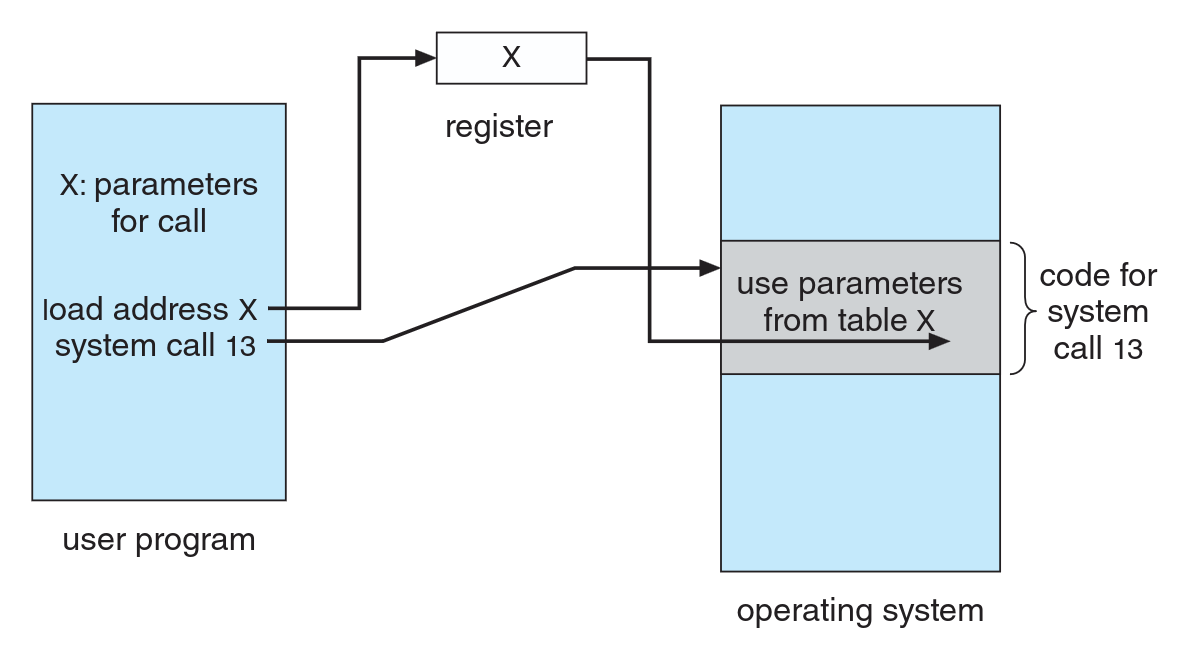
\includegraphics[width=0.8\linewidth]{Images/calls/param.png}
    \caption{Esempio di Passaggio di Parametri.}
\end{figure}

\subsection{Tipi di Chiamate di Sistema}
Esistono sei tipi di system calls:
\begin{enumerate}
  \item \textbf{Process Control}:
    \begin{enumerate}
      \item Creazione e terminazione di processi;
      \item Caricamento ed esecuzione;
      \item Eventi e segnali di wait;
      \item Allocazione e liberazione della memoria;
      \item Get e set di attributi dei processi.
    \end{enumerate}
  \item \textbf{File Management}
    \begin{enumerate}
      \item Creazione ed eliminazione di file;
      \item Apertura e chiusura di file;
      \item Lettura e scrittura di file;
      \item Get e set di attributi dei file.
    \end{enumerate}
  \item \textbf{Device Management}:
    \begin{enumerate}
      \item Richiesta e rilascio un dispositivo;
      \item Lettura e scrittura;
      \item Get e set degli attributi di un dispositivi;
      \item Attach e detach logico di dispositivi.
    \end{enumerate}
  \item \textbf{Information Maintenance}:
    \begin{enumerate}
      \item Get e set di tempo e data;
      \item Get e set di dati di sistema;
      \item Get e set di attributi di file, processi e dispositivi.
    \end{enumerate}
  \item \textbf{Communications}:
    \begin{enumerate}
      \item Creazione ed eliminazione canali di comunicazione;
      \item Invio e ricezione di messaggi;
      \item Trasferimento di informazioni di stato;
      \item Attach e detach di dispositivi remoti.
    \end{enumerate}
  \item \textbf{Protection}:
    \begin{enumerate}
      \item Get file permission;
      \item Set file permission.
    \end{enumerate}
\end{enumerate}

\section{Servizi di Sistema}
\begin{defn}[Servizi di Sistema]
Offrono un ambiente conveniente per programmare ed eseguire applicazioni. \\ 
Alcuni sono solamente warp di chiamate di sistema, altre invece sono più complessi.
\end{defn}
Ci sono diverse categorie:
\begin{itemize}
  \item \textbf{Gestione dei file:} permettono di eseguire diverse operazioni su file e directory.
  \item \textbf{Informazioni di Status:} permettono di interrogare l'SO per avere informazioni come data, tempo, spazio su memoria o dischi, ecc... \\ 
    Inoltre, permettono azioni più complesse come il logging, il debugging e l'analisi di prestazioni.
  \item \textbf{Modifica dei File:} modificare o creare file su dischi, tramite, per esempio, svariati text editor.
  \item \textbf{Supporto a linguaggi di Programmazione:} Compilatori, debugger e interpreti per linguaggi di programmazione tipo C/C++, Java, Python, ecc...
  \item \textbf{Esecuzione e Caricamento dei Programmi:} i programmi devono essere caricati in memoria ed eseguiti. Il sistema deve fornire linker e loader, oltre a i vari debugger.
  \item \textbf{Comunicazioni:} permettono di creare canali di comunicazioni virtuali fra processi, utenti o computer.
  \item \textbf{Servizi di Bakcground:} alcuni servizi vengono lanciati nel tempo di boot, alcuni terminano, altri invece continuano a lavorare finchè il sistema non viene spento. \\ 
    Normalmente, quest'utlimi sono chiamati \textbf{demoni}.
\end{itemize}

\section{Linker e Loaders}
Solitamente, un programma per essere eseguito da una CPU deve essere caricato nella memoria centrale e metto in lista come processo. Per fare questa cosa sono necessari diverse fasi. \\

\begin{figure}[!htb]
    \centering
    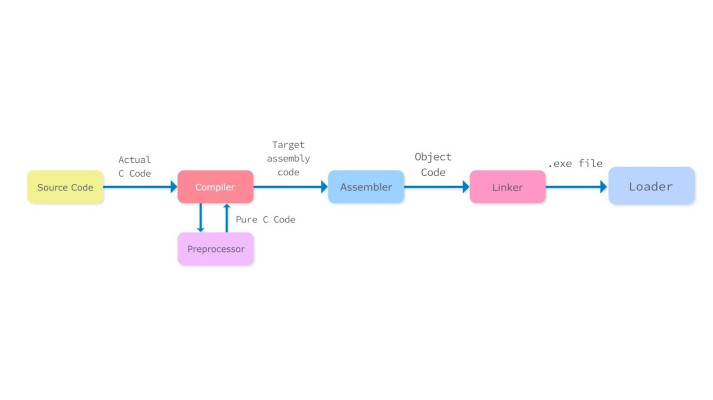
\includegraphics[width=0.5\linewidth]{Images/calls/programm.jpg}
    \caption{Ciclo completo di un programma C.}
\end{figure}

Per prima cosa, il programma viene compilato in un file oggetto per essere caricato in una memoria fisica. Questo formato è chiamato \textbf{file oggetto reallocabile}. \\ 
Successivamente, il \textbf{linker} combina i vari file oggetto e le librerie necessarie in un unico file eseguibile. \\ 
Infine, il \textbf{loader} si occupa di caricare il programma in memoria centrale per essere eseguito dalla CPU. Un'attività importante di questa fase è la \textbf{riallocazione}, dato che è necessario assegnare un indirizzo finale alle varie parti del programma, ai dati e pure al codice. \\
\vspace*{0.01\textheight}
I file oggetto e i file eseguibili presentano solitamente formati standard che includono il codice macchina compilato e una tabella dei simboli contenente metadati relativi a funzioni e variabili a cui il programma fa riferimento. 
Per i sistemi UNIX e Linux, questo formato standard è noto come \textbf{ELF} (\textbf{Executable and Linkable Format}).

\begin{ex}[Formato ELF]
Con il comando \texttt{file} è possibile identificare e valutare i formati ELF. \\ 
Per esempio con: 
\[
  \texttt{file main.o} \\ 
\]
verrà riportato che il \texttt{main.o} è un file ELF reallocabile.\\ 
Invece: 
\[ 
  \texttt{file main} \\
\]
riporterà che \texttt{main} è un file ELF eseguibile.
\end{ex}
